% !TEX root = ../thesis.tex
%
\chapter{Results and Evaluation}
\label{sec:evaluation}

In this section, we will present and interpret the results of our experiments as presented in Chapter~\ref{sec:experiments}.
This involves firstly a brief analysis of the results of the original STAMP benchmark to establish them as a baseline to legitimize or discuss the results of our Rust-based STM implementation of the algorithm as we will use the latter to evaluate Ohua's performance.
Subsequently, we will analyze the results of our Ohua benchmarks in detail to see, whether it could be used as a suiting replacement for STM in terms of performance.


\section{Reference Measurement Results}

\begin{figure}
    \centering
    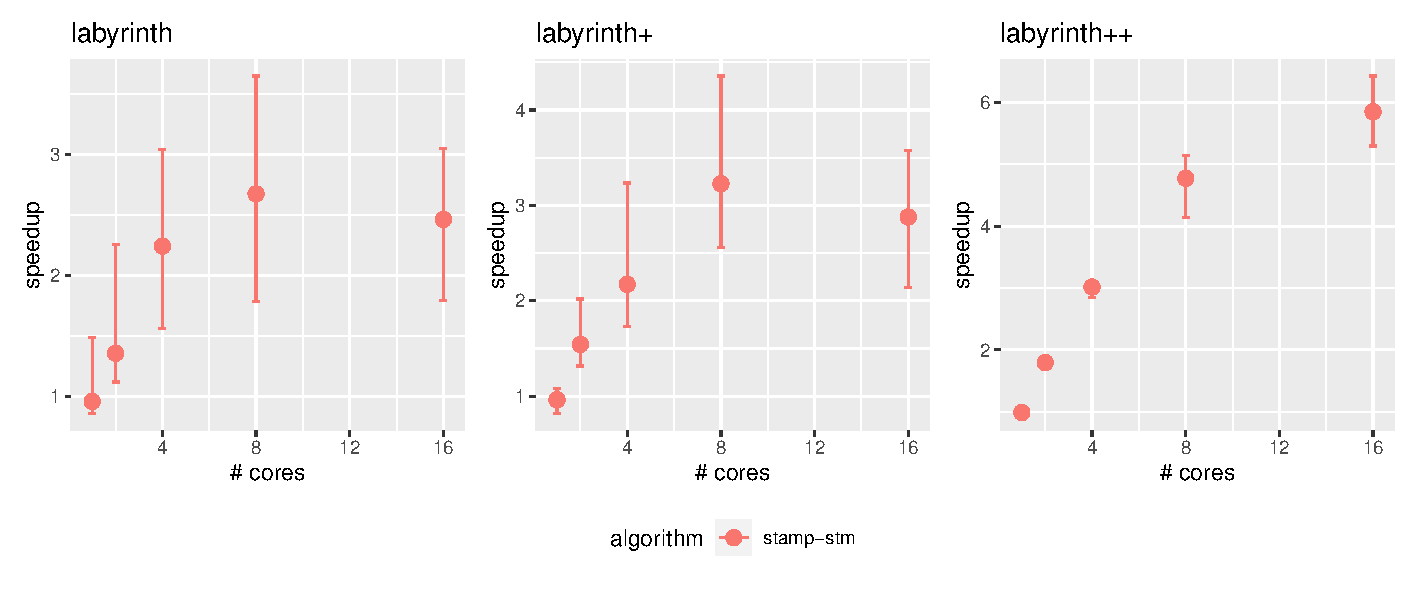
\includegraphics[width=\textwidth,keepaspectratio]{gfx/results/stamp/stamp_labyrinth_comb}
    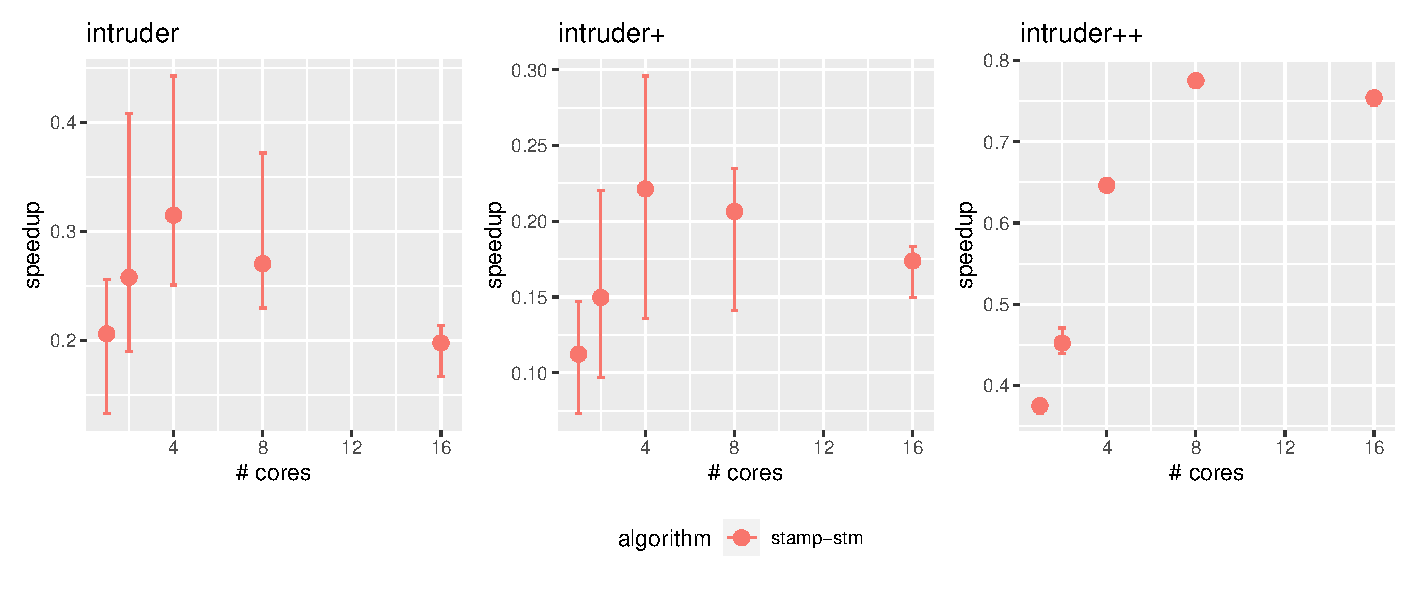
\includegraphics[width=\textwidth,keepaspectratio]{gfx/results/stamp/stamp_intruder_comb}
    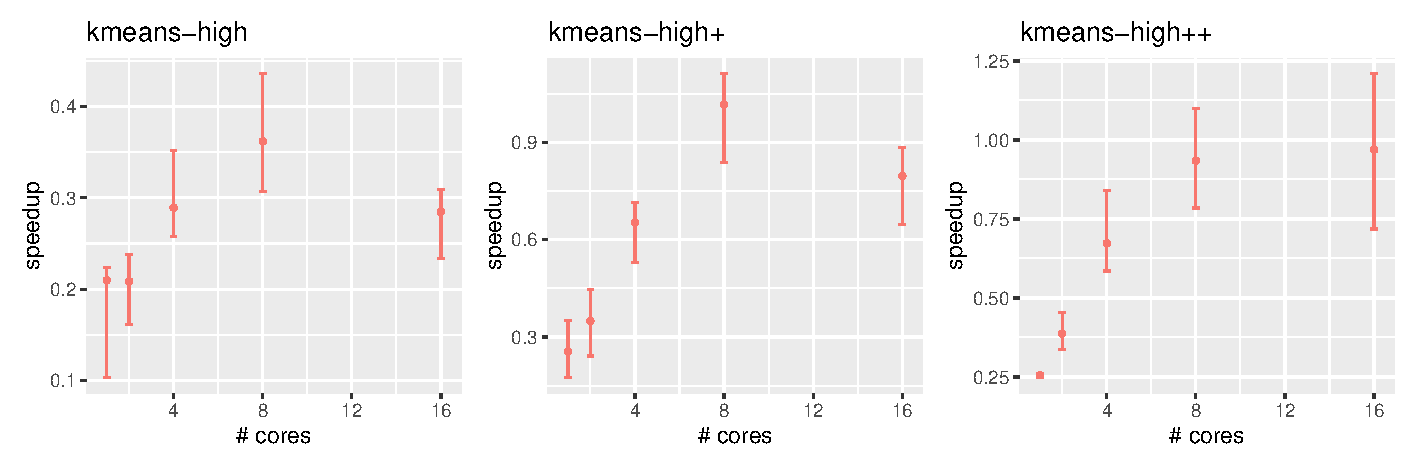
\includegraphics[width=\textwidth,keepaspectratio]{gfx/results/stamp/stamp_kmeans-high_comb}
    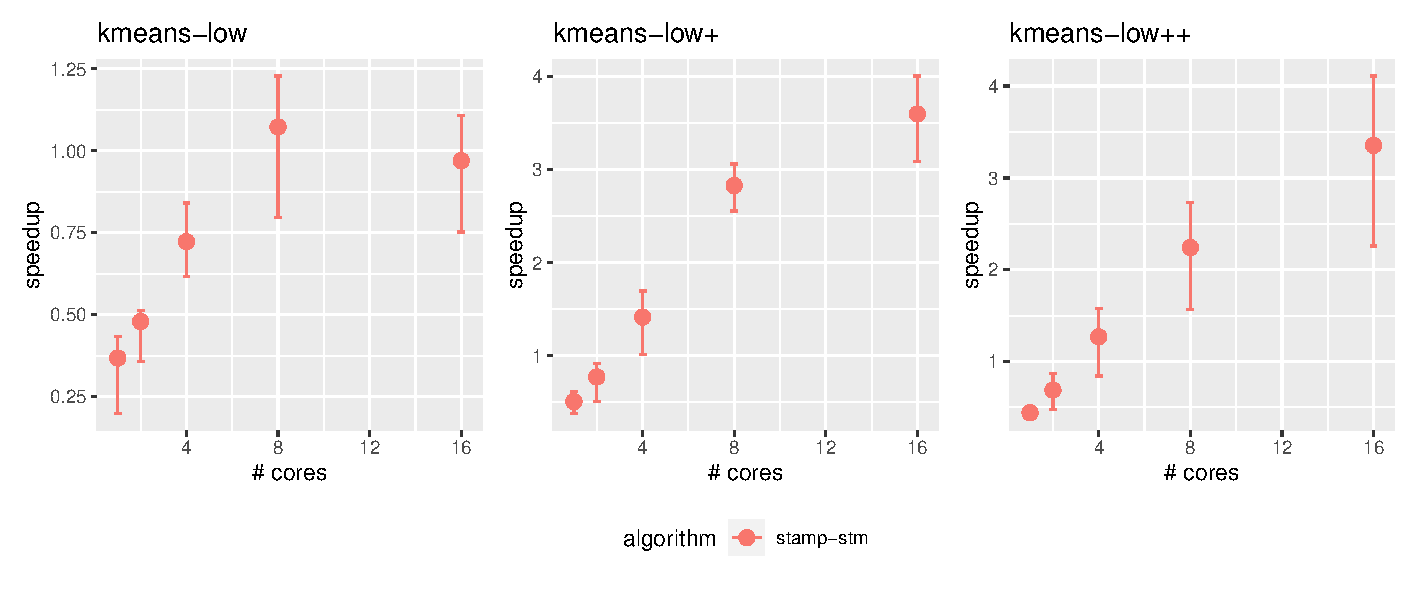
\includegraphics[width=\textwidth,keepaspectratio]{gfx/results/stamp/stamp_kmeans-low_comb}
    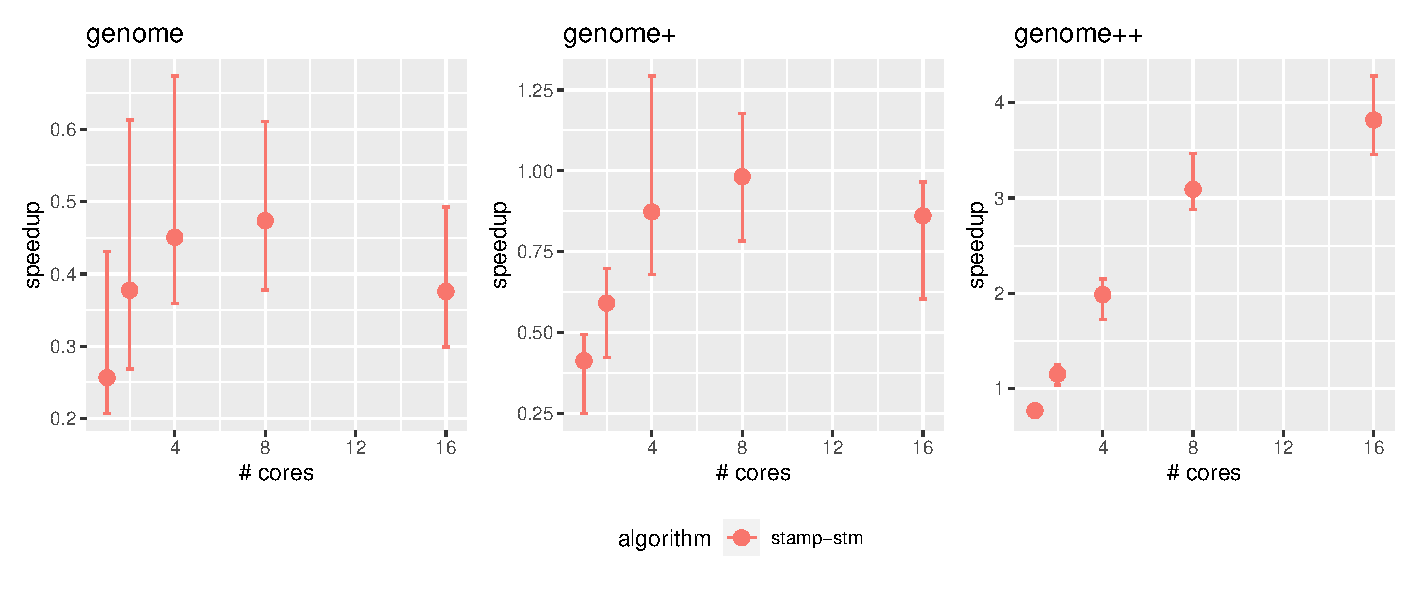
\includegraphics[width=\textwidth,keepaspectratio]{gfx/results/stamp/stamp_genome_comb}
    \caption{Speedup achieved by STM in the original STAMP  benchmarks.}%
    \label{fig:evaluation:stamp}
\end{figure}

Benchmark results for the reference measurement runs we conducted can be found in Figure~\ref{fig:evaluation:stamp}.
We will compare our achieved speedups to the original benchmark runs from Minh et al.~\cite{minh2008stamp}, namely to the results of their Eager STM implementation to see, how performance of the framework changed over the years.
This allows us to set realistic expectations for the performance of our STM-based implementations.

In the \emph{labyrinth} benchmark, we observed an increasing speedup for up to 8 threads in the small and medium sized problem sets, maxing at about 3.0 speedup and followed by declining performance for 16 threads.
The largest input data set on the other hand exhibits a steadily increasing curve, achieving a speedup of about 6.0 for 16 threads.
This deviates from the original results, where both the labyrinth and the labyrinth+ benchmark showed behavior similar to our labyrinth++ curve form: A continuously increasing performance, achieving a speedup of about 4.0 at best.
The form of the curve and the overall reduced performance may indicate that either the sequential implementation is performing better now than it did back in 2008 or that the overhead of the \texttt{tl2} STM framework increased.
Our first theory is backed as possible cause by the fact that compiler optimizations have improved in the past years along with CPU clock speeds, making a better sequential performance not unlikely.
An increased framework overhead on the other hand would also support the performance drop for 16 threads, which the better sequential performance does not explain.
This was also discussed previously by Perfumo et al.~\cite{perfumo2008limits} who reported similar performance drops for STM applications with higher thread counts.
Another explanation for this decline would be our used hardware architecture, as it consists of two CPUs.
While all runs up to 8 threads can be executed on a single CPU, the 16 thread version requires the utilization of both cores, requiring more complex memory and resource management which in turn takes more time and may also be an explanation since we do not know if Minh et al.\ had similar hardware.
But since we only made this and the following measurements as reference points for the data we acquired in our own experiments, we did not investigate the causes for this behavior beyond speculations to possible reasons and leave this to future work.

A similar deviation from the original measurements can be seen for the \emph{intruder} application.
Our own results show a curve that peaks at 4 or 8 threads respectively, before declining again.
Maximum speedups are as low as 0.3 for the small, about 0.2 for the medium and 0.8 for the largest input set.
The original results on the other hand show Eager STM achieving a speedup slightly below 1 for both intruder and intruder+\footnote{Hardware-based Transactional Memory approaches perform generally better in this benchmark.} meaning that our results are again remotely similar, taking into account our previous assumptions about possible changes in the execution environment compared to the original benchmarks.

For its high-contention scenario, our \emph{kmeans} measurements show a similar behavior as the previous applications.
Both smaller benchmarks achieve peak performance for 8 threads while performance decreases for 16 threads or stagnates in the case of kmeans-high++.
In the original measurements however, the authors achieved steadily increasing near-linear speedups like our high++ version did with speedups of up to 4.0 for both input sets while we only achieved a maximal speedup of 1.0 for both high+ and high++.\\
A more stark deviation is visible in the low-contention variant of the benchmark:
The original speedup grew linearly with increasing number of threads used due to the low contention, maxing out at execution times 9 or 10 times faster than the sequential version respectively.
We again have a peak performance at 8 threads for the kmeans-low variant but steadily increasing speedups for low+ and low++, achieving a 3.5 speedup.

In \emph{genome}, we achieved for the first time curve shapes similar to the original results from Minh et al., although the original results showed peak performance at 4 threads while our results peak at 8 threads before decreasing again.
Also, our total achieved speedup is slightly below the originally reported numbers.
The solid performance of genome++ might be due to the fact that the overhead of the used framework amortized for this large input set.

Overall, our results are remotely similar to the original results, although we consistently observed lower speedups than reported in the original.
We identified either a better sequential performance, increased framework overhead or hardware overhead as possible sources, in reality it may even be a combination of all these factors.
Due to the fact that both result sets vary greatly, we opted to discard the original results reported by Minh et al.\ in favor of using our own measurements as reference for our Rust-STM implementations.


\section{Rust-based Benchmark Results}%
\label{sec:evaluation:benchmarks}

\begin{figure}
    \centering
    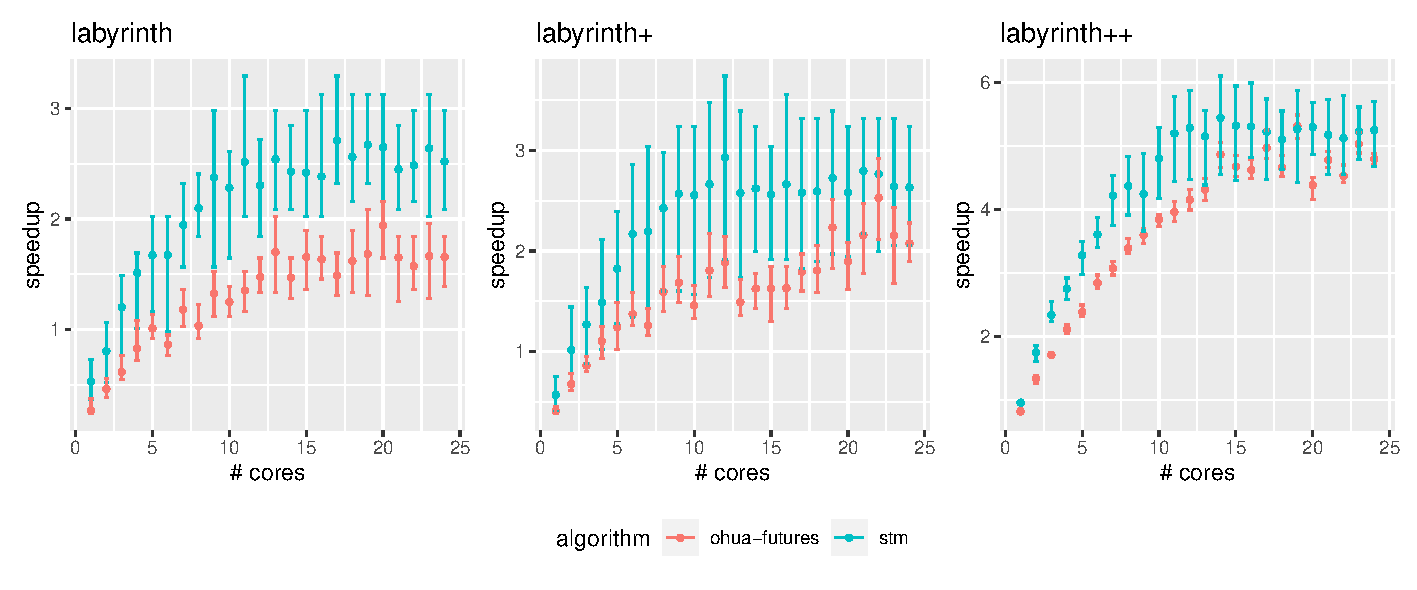
\includegraphics[width=\textwidth,keepaspectratio]{gfx/results/labyrinth_comb}
    \caption{Speedup in the labyrinth application relative to a sequential implementation.}%
    \label{fig:evaluation:labyrinth}
\end{figure}

\paragraph{labyrinth.} We already discussed in detail the performance of the \emph{labyrinth} application for Ohua and STM, which is shown in Fig.~\ref{fig:evaluation:labyrinth}, in Chapter~\ref{sec:preliminary}.
Notably, Ohua performs slightly worse than STM, but shows the same overall scaling behavior for more cores while exhibiting less variance in the results.
For labyrinth++, one can not state clearly, which benchmark performs better due to the comparatively large variance in the STM results.
The Software Transactional Memory implementation itself performs just as the original STAMP implementation by Minh et al.~\cite{minh2008stamp}, reinforcing the validity of our implementation.

\begin{figure}
    \centering
    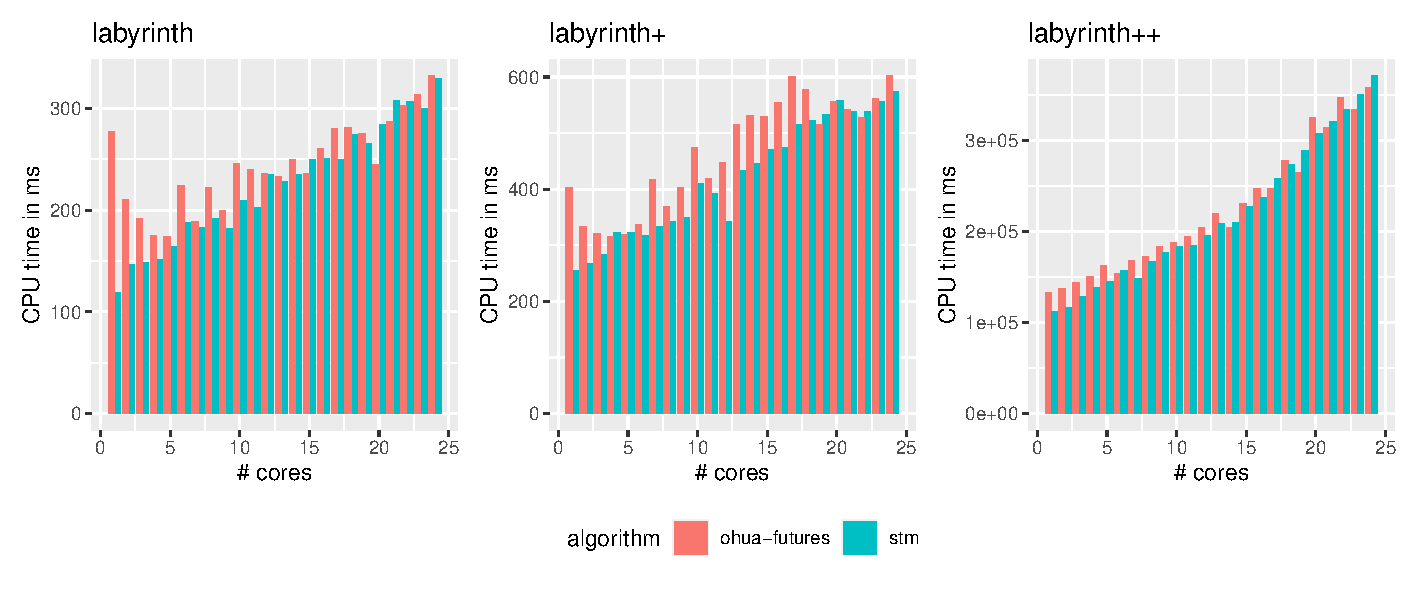
\includegraphics[width=\textwidth,keepaspectratio]{gfx/results/cpu_labyrinth_comb}
    \caption{CPU time used by both frameworks in the labyrinth application.}%
    \label{fig:evaluation:labyrinth-cpu}
\end{figure}

When comparing the CPU time used by both Ohua and STM as shown in Figure~\ref{fig:evaluation:labyrinth-cpu}, we unsurprisingly see an overall growing demand for computation time as creating more threads and moving data between them in itself takes more time.
One can observe the correlation between the time spikes for both applications in the labyrinth+ benchmark and a degraded performance for the respective thread counts.
Due to Ohua's algorithm structure, low thread counts become even less performant for smaller input sets, as fewer threads require more loops of the algorithm, creating a non-negligible runtime overhead.
This becomes irrelevant for larger inputs such as labyrinth++, though.


\begin{figure}
    \centering
    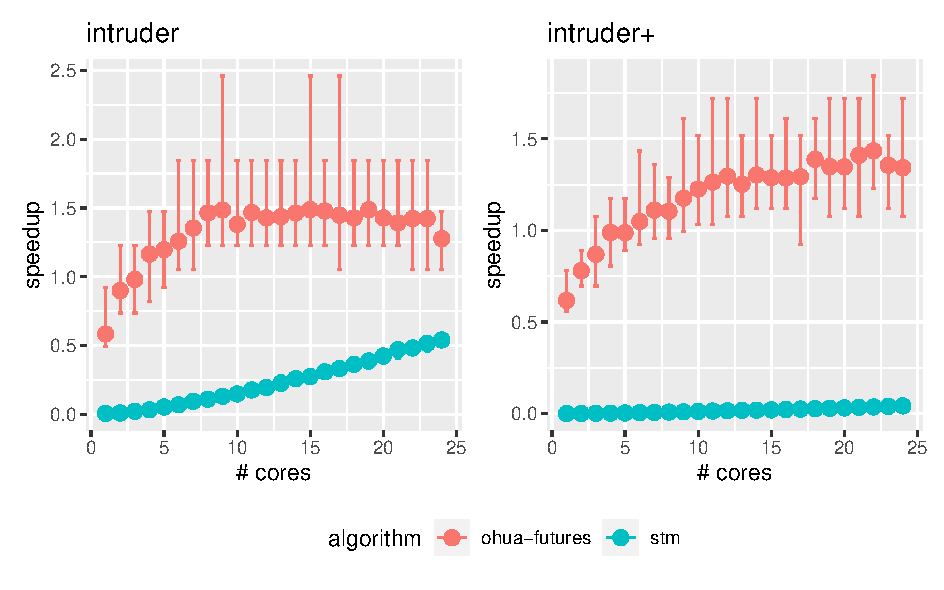
\includegraphics[width=\textwidth,keepaspectratio]{gfx/results/intruder_comb}
    \caption{Speedup in the intruder application relative to a sequential implementation.}%
    \label{fig:evaluation:intruder}
\end{figure}

\begin{figure}
    \centering
    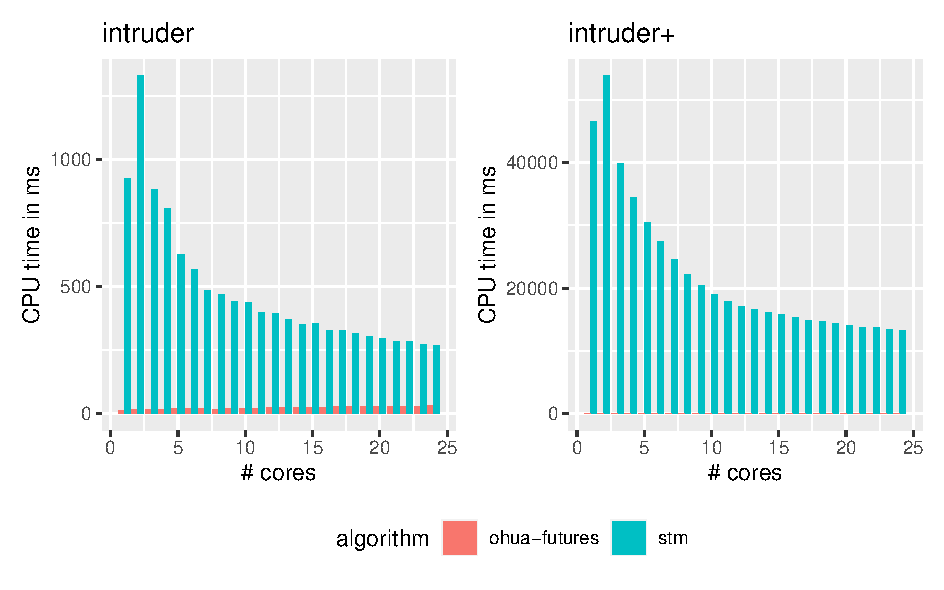
\includegraphics[width=\textwidth,keepaspectratio]{gfx/results/cpu_intruder_comb}
    \caption{CPU time used by both frameworks in the intruder application.}%
    \label{fig:evaluation:intruder-cpu}
\end{figure}

\paragraph{intruder.} For the \emph{intruder} program, both frameworks deliver extremely different results:
STM performance for the small input set (as seen in Fig.~\ref{fig:evaluation:intruder}) is similar to the performance showcased in the reference measurements in Fig.~\ref{fig:evaluation:stamp}, although the curve shape is different, the Rust version showing a slow and steady increase in performance.
The medium sized input set however, produces a rise so flat it almost becomes invisible due to the graph scaling.
We suspect this to be caused by the slow reassembly phase of the benchmark, which operates on a shared HashMap.
Even though we augmented the standard libraries' HashMap implementation with basic transaction handling capabilities like Minh et al.\ did, there is still a lot of contention on these shared data instances, impacting execution times.
This assumption is supported by the immense amount of CPU time used by the STM implementation.
Because of these long execution times we did not measure STM's speedups for the significantly larger intruder++ input set.

Ohua on the other hand achieves in both smaller cases relatively good speedups of about 1.5 and 1.3 respectively, outperforming Software Transactional Memory.
Particularly interesting is the performance plateau that is reached by Ohua for a medium amount of threads and which is best visible in the smallest input set.
Source of this is the fact that a not insignificant portion of the algorithm runs sequentially in Ohua, as explained in Chapter~\ref{sec:experiments:intruder}.
Hence, only a certain speedup may be achieved by parallelizing the application, thus creating a plateau that transitions into declining performance later on when the framework overhead becomes too large.
But as was the case with STM, the intruder+ version performs slightly worse than the smaller input set and Ohua's intruder++ results are even worse, below 1.0.
This can be attributed to the increasing input set sizes, which take longer to process during the sequential flow reassembly phase, impairing the speedup achieved by the parallel detection phase.
The aforementioned performance difference is also clearly seen in the use of CPU time which is shown in Figure~\ref{fig:evaluation:intruder-cpu}, where Ohua uses orders of magnitude less CPU time than STM.

\paragraph{kmeans} Our \emph{kmeans} results show no clear winner in terms of performance.
Although there were differences in the performance behavior between the high contention and low contention versions of the STAMP benchmark, the STM version written in Rust showcases in Figures~\ref{fig:evaluation:kmeans-high} and~\ref{fig:evaluation:kmeans-low} similar curve shapes for both sets of input data which are completely different from the results in Fig.~\ref{fig:evaluation:stamp}.
This is most likely due to differences in the implementations of both benchmark versions.
C-based programs allow ways of memory sharing that are irreproducible in Rust, forcing us to change some aspects of the program, probably causing these differences.
An example for the differences in what is considered legal memory sharing can be seen in the following snippet of C code:
\begin{minted}{C}
    unsigned long data[] = {1, 2, 3, 4, 5, 6, 7, 8, 9, 10};

    pid_t pid = fork();
    if (pid != 0) {
        int lower = 0;
        int upper = 4;
        // changes elements at indices 0 to 4
        modify_elements(data, lower, upper);
    } else {
        int lower = 5;
        int upper = 9;
        // changes elements at indices 5 to 9
        modify_elements(data, lower, upper);
    }
\end{minted}
There, an array of data (in this example integers, but in \emph{kmeans} it would be observations to classify) is to be manipulated by two concurrent threads.
Since the developer wants to split the work evenly between both threads, she can assign both threads non-overlapping ranges to iterate over and let both threads work directly on the array.
Without any locking, this is risky, as there is no control mechanism ensuring that both threads don't alter the memory regions of the other thread due to a bug in an index calculation or by writing too large portions of data to the array.
Nonetheless, this is the fastest possible implementation (due to the absence of safeguards).
In Rust however, this is impossible.
The language itself does not allow this type of fast yet unsafe memory sharing, as the type system ensures that data shared across threads without locks is read-only.
So, if one wants to implement the same algorithm shown in above listing without locks in Rust, the data must either be copied\footnote{In Rust jargon, this is called a \emph{clone}.} and sent to the respective threads (making a later consolidation of the changes made necessary) or the vector has to be split apart, each part moved into the scope of the respective thread.
Both approaches are time-consuming, as in both cases new memory must be allocated for the new vectors and the data has to be copied or moved, not to mention the time it takes to consolidate the changes made afterwards.

\begin{figure}
    \centering
    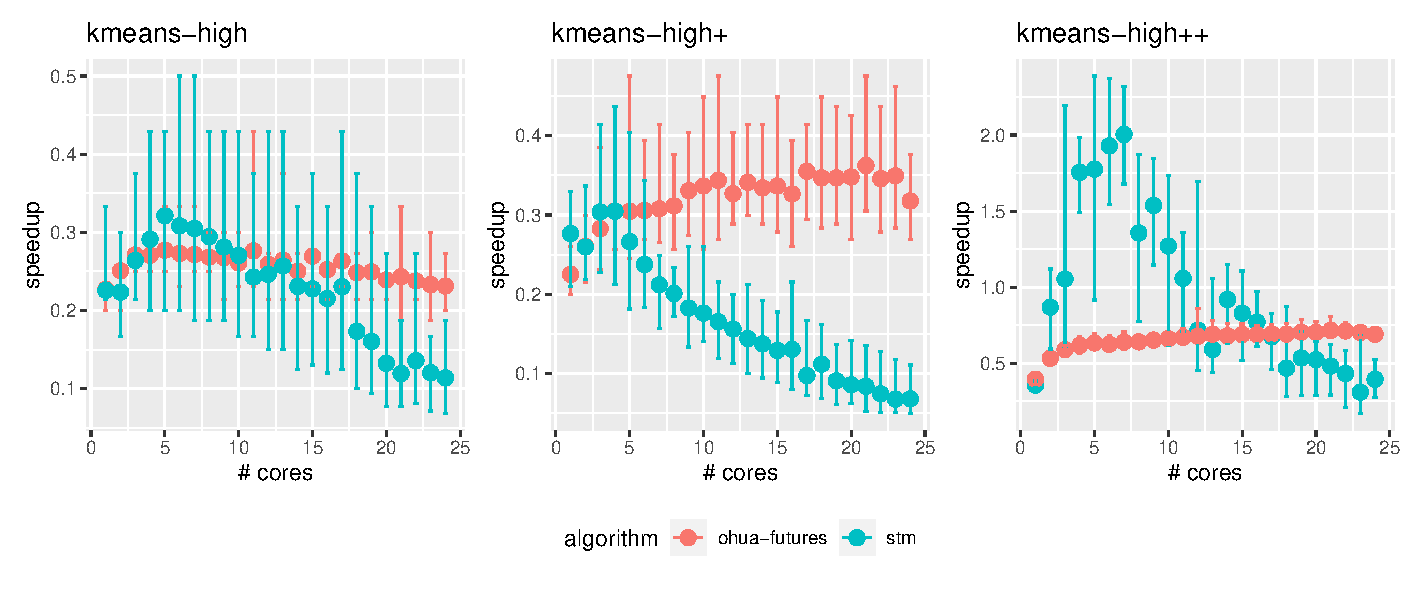
\includegraphics[width=\textwidth,keepaspectratio]{gfx/results/kmeans-high_comb}
    \caption{Speedup in the kmeans-high application relative to a sequential implementation.}%
    \label{fig:evaluation:kmeans-high}
\end{figure}

\begin{figure}
    \centering
    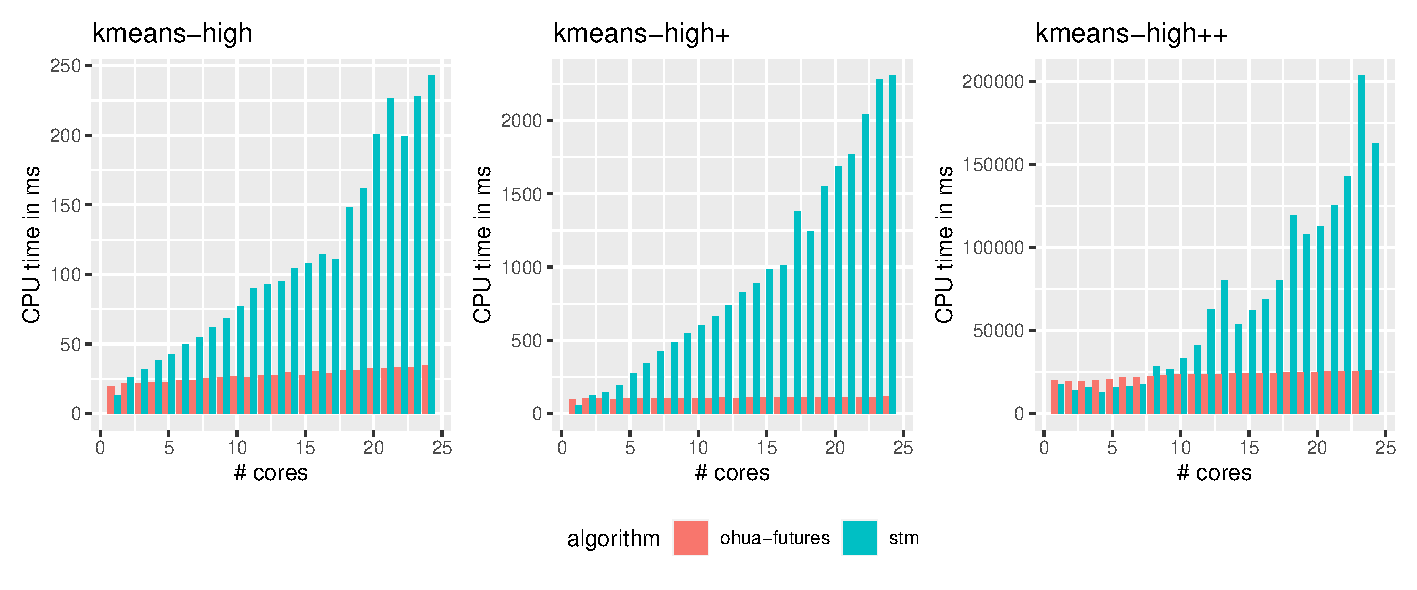
\includegraphics[width=\textwidth,keepaspectratio]{gfx/results/cpu_kmeans-high_comb}
    \caption{CPU time used by both frameworks in the kmeans-high application.}%
    \label{fig:evaluation:kmeans-high-cpu}
\end{figure}

Overall, both benchmark sets show that there is no clear pattern for Ohua's performance with respect to the size of the input set.
Each individual set of input data requires a specific number of iterations before the algorithm converges.
In the Software Transactional Memory version this number is completely unpredictable, fluctuating due to the order in which the elements are processed, as floating point addition offers only a limited precision and is hence not commutative.
Minor differences in the calculation of new centroids therefore can lead to missing the convergence threshold which in turn leads to more computations.
Ohua does this in a fixed amount of iterations as it performs all additions deterministically.
This becomes visible in Ohua's fairly level performance for each input set.
As its determinism guarantees that the computations performed are always in the same order, stripped of any fluctuations caused by non-determinism, speedups and slowdowns mark where the framework either helps to improve performance or where it weighs down execution times.

\begin{figure}
    \centering
    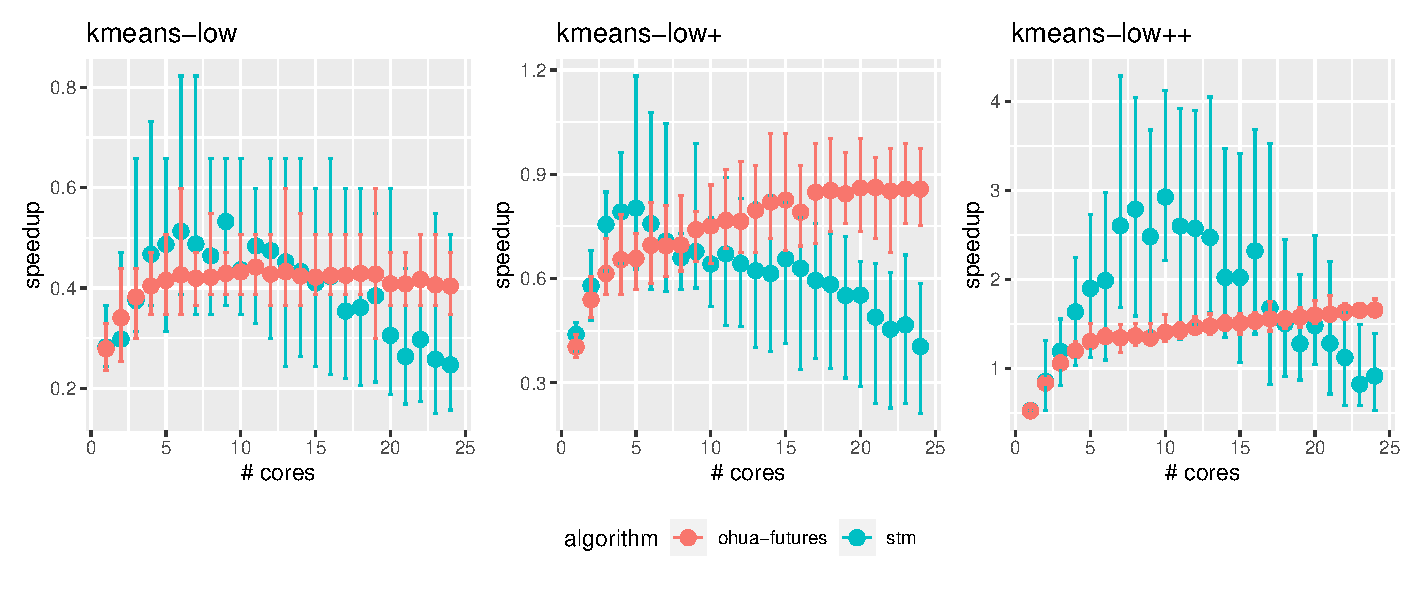
\includegraphics[width=\textwidth,keepaspectratio]{gfx/results/kmeans-low_comb}
    \caption{Speedup in the kmeans-low application relative to a sequential implementation.}%
    \label{fig:evaluation:kmeans-low}
\end{figure}

\begin{figure}
    \centering
    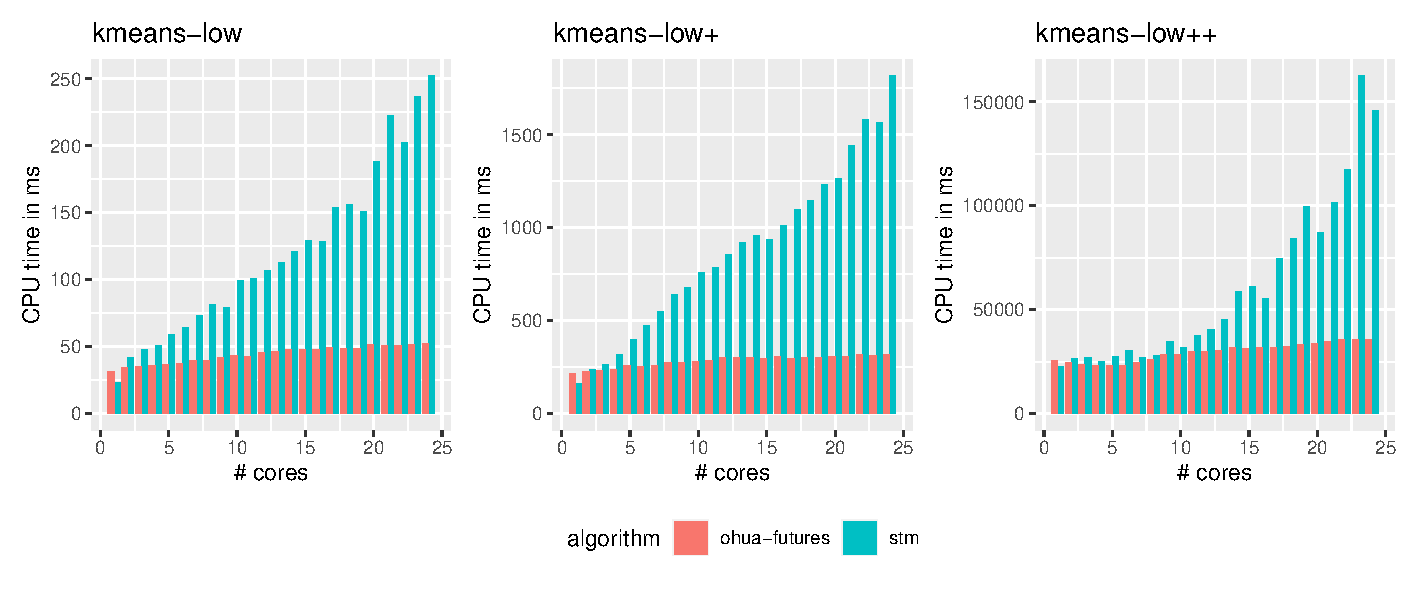
\includegraphics[width=\textwidth,keepaspectratio]{gfx/results/cpu_kmeans-low_comb}
    \caption{CPU time used by both frameworks in the kmeans-low application.}%
    \label{fig:evaluation:kmeans-low-cpu}
\end{figure}

When comparing the utilized CPU times by both frameworks in Figs.~\ref{fig:evaluation:kmeans-high-cpu} and \ref{fig:evaluation:kmeans-low-cpu}, we see that Ohua uses a relatively steady amount of computation time throughout all measurements for kmeans, while STM needs linearly more computation times with increasing thread count.
This can be attributed to an increased number of conflicts due to higher contention, the latter also showing in degrading speedups with increasing thread counts.
All in all, Ohua is on par or outperforms Software Transactional Memory in the smaller two of both kmeans input sets and performs steadily for both large inputs, all while utilizing only a fraction of the CPU time STM needs, meaning it is also using significantly less energy to produce its results.

\begin{figure}
    \centering
    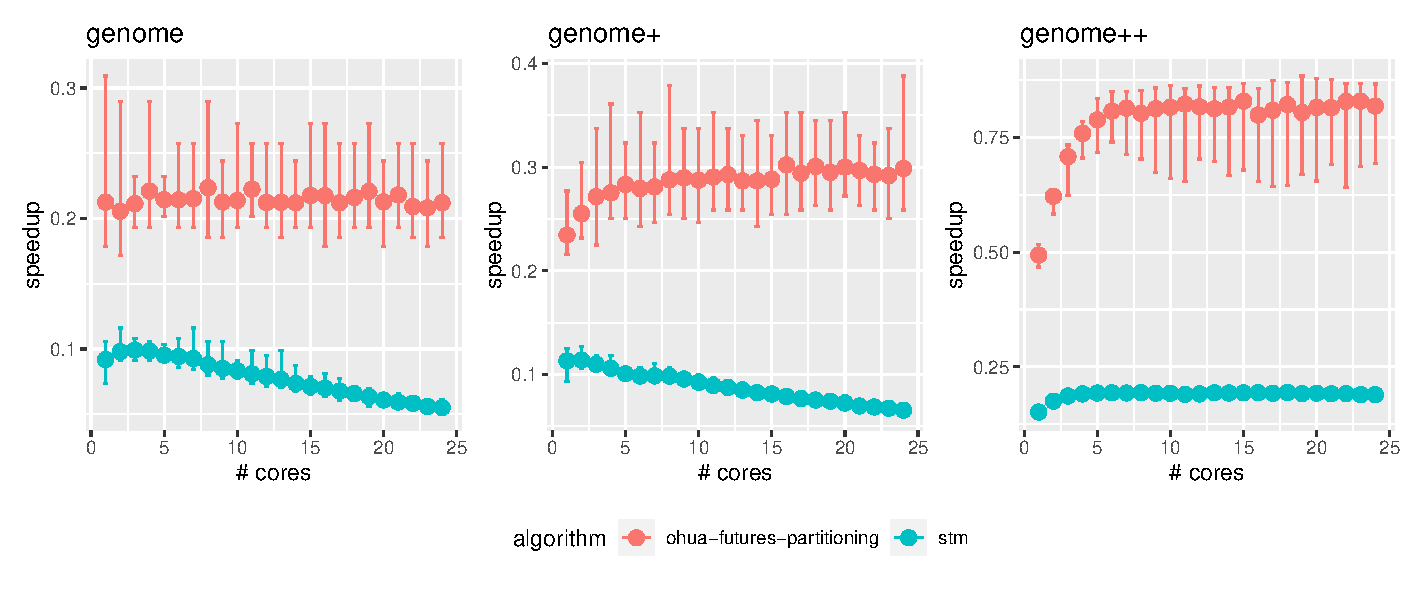
\includegraphics[width=\textwidth,keepaspectratio]{gfx/results/genome_comb}
    \caption{Speedup in the genome application relative to a sequential implementation.}%
    \label{fig:evaluation:genome}
\end{figure}

\newpage

\paragraph{genome.} In \emph{genome}, the curve shapes of our STAMP results from Fig.~\ref{fig:evaluation:stamp} and the results from the STM version in Rust in Fig.~\ref{fig:evaluation:genome} are similar in the way that they exhibit peak performance for a medium amount of threads before it declines.
What's striking is the difference in absolute speedups achieved by our Rust implementation.
Likely causes for this include a by comparison more performant sequential implementation, which is possible as we developed these binaries independently from the other implementations which use one of the two frameworks while Minh et al.\ basically reuse the STM implementation, only removing any TM and threading code from it.
Alternatively, it could be because of higher overheads of the \texttt{rust-stm} library, for reasons we have outlined above.
To test this theory, we profiled a STM \texttt{genome+} run using 8 threads and analyzed the resulting flamegraph~\cite{gregg2016flame}.
We found that the cloning of data amounts for about 23,75 \% of the whole execution time of the benchmark\footnote{For this analysis we profiled the whole application execution. Of the overall execution time, only 46,06 \% of all samples were attributed to the execution of the benchmark itself. 10,94 \% of the total sample count were attributed to data cloning and also within the benchmark execution part of the program. Hence, roughly 23,75 \% of the benchmark execution time is spent duplicating data.}.
While a more efficient library implementation using Rust's \emph{unsafe} features that allow circumventing certain safeguards could may help to improve performance, we deemed time-consuming improvements on a STM framework out of scope for this work.
Ohua manages to achieve clearly better speedups in all three test cases.
The execution times remain relatively similar, indicating a steady amount or overhead, although we see an increasing CPU usage in Figure~\ref{fig:evaluation:genome-cpu}, indicating the increasing framework overhead.
But due to the large portions of still sequential code, i.e., the nucleotide sequence deduplication, no real performance gains can be made.

\begin{figure}
    \centering
    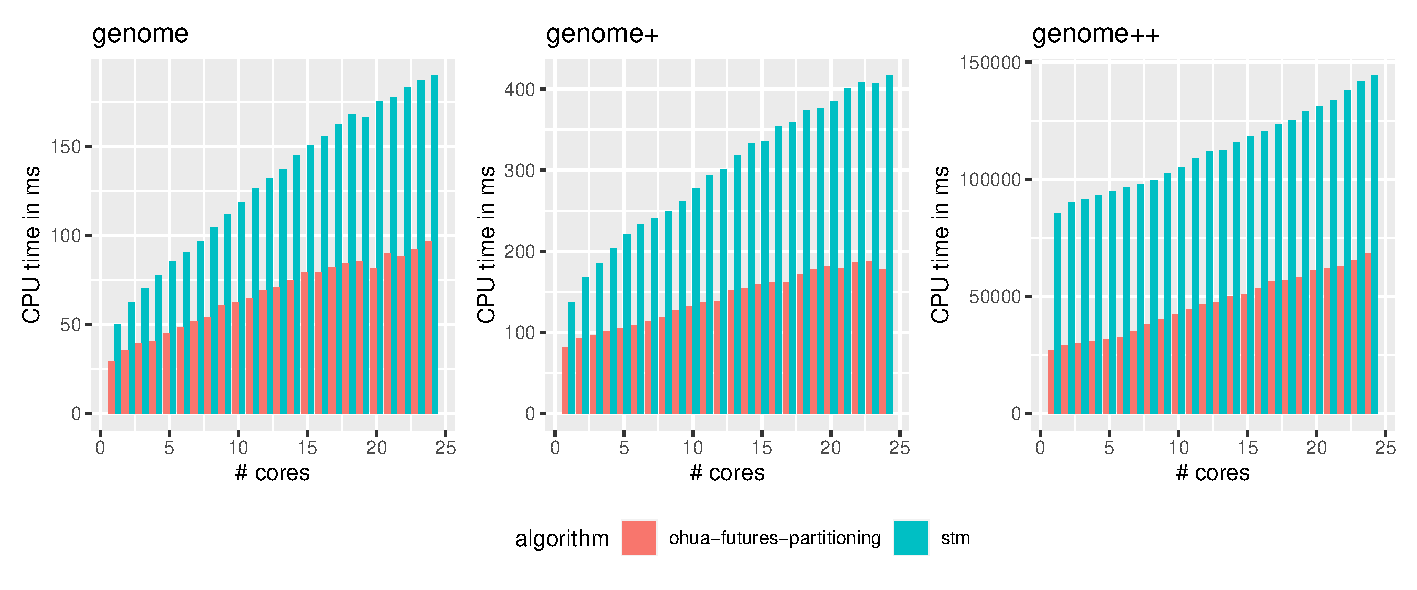
\includegraphics[width=\textwidth,keepaspectratio]{gfx/results/cpu_genome_comb}
    \caption{CPU time used by both frameworks in the genome application.}%
    \label{fig:evaluation:genome-cpu}
\end{figure}


\section{Summary}%
\label{sec:evaluation:summary}

In general, the experiments we've conducted have shown that Ohua's deterministic execution model does indeed lead to less variance in execution times. %\footnote{This is not immediately visible in the speedup plots in Chapter~\ref{sec:evaluation:benchmarks}, due to the formula used to determine speedup.}.
Our achieved results are on par with those of STM in applications like the labyrinth benchmark, where it was able to break up the stateful loop using Transformation~2 and~3.
Technically, we also outperformed Software Transactional Memory in the intruder and genome benchmarks but as STM achieved in both cases subpar results, it should be evaluated whether the STM library used can be optimized for a performance comparable to the C-based version or whether this is not an implementation-related but rather a framework-related issue before judging about this.

With the kmeans and genome benchmarks, it became apparent that not all shared state applications offer the same amount of parallelism exploitable using the transformations we proposed in Chapter~\ref{sec:transformations}.
In fact, it became apparent that of the various forms of irregular applications tested, the one exhibiting amorphous data parallelism could be parallelized best: the labyrinth benchmark.
This is the only one of the four algorithms we implemented that displays the characteristics of amorphous data parallelism we explained in Chapter~\ref{sec:background:irregular:adp}.
That may indicate that Ohua would be most effective when targeting this type of applications in particular, as our batching Transformation~2 and~3 presented in chapters~\ref{sec:transformations:tf15} and~\ref{sec:transformations:tf2} enable us to handle the state updates found in this type of applications.
To verify this, future work should implement other programs from the STAMP suite that contain amorphous data parallelism such as the \emph{yada} and \emph{ssca2} algorithms.
But even in the non-amorphous cases we tested Ohua on, we saw a significantly lower CPU usage, and by extension power consumption, for Ohua than for STM.
The absence of contention in Ohua's model is the key reason for this conservation of resources.
Hence, the fact that the framework is more limited in what parallelism may be exploited does not seem to be a downside but rather an advantage.
Such state-modification-only loops contain usually more contention as transactions are much shorter and commits occur more frequently.
Exploiting parallelism from these loops hence has the potential of yielding a negative instead of a positive performance impact, as more write conflicts and recomputations occur.

Overall, Ohua would indeed seem to be a promising replacement for STM-based shared state applications.
While it is clearly not suited to be used for every type of shared state program, so is STM.
Performance-wise Ohua will not always outperform Software Transactional Memory but manages to at least be on par with it, while yielding other positive properties like a deterministic execution model, often better energy efficiency, and easier to work with code bases due to the elimination of parallelism abstractions.
Based on the benchmark results we assume, that Ohua will showcase the best performance behavior when used in applications with amorphous data parallelism as this allows it to not just parallelize state-free loops but also stateful loops using Transformation~2 and~3.

% - present benchmark results -- maybe for the manual Ohua implementation as well, if results differ
% - discuss why we perform better/worse at certain points
% - we see the determinism!
% - discuss energy usage etc
